\documentclass[]{article}
\usepackage[MeX]{polski}
\usepackage[utf8]{inputenc}
\usepackage{graphicx}
\usepackage{xcolor}
\usepackage{float}
\usepackage{ulem}
\usepackage{placeins}
\title{TECY - Projekt 1}
\author{Małgorzata Pszczółkowska - 311423\\ Anastasiya Ronskaya - 317058 \\ Konrad Kotlicki - 310958 \\Sebastian Skrzek - 311442}
\begin{document}
\maketitle
\tableofcontents
\section{Wskaźnik}
Nasz wskaźnik do danych to:
$3+8+8+2=2\textbf{\underline{1}}$
\section{Tablica funkcji}
\begin{figure}[H]
	\centering
	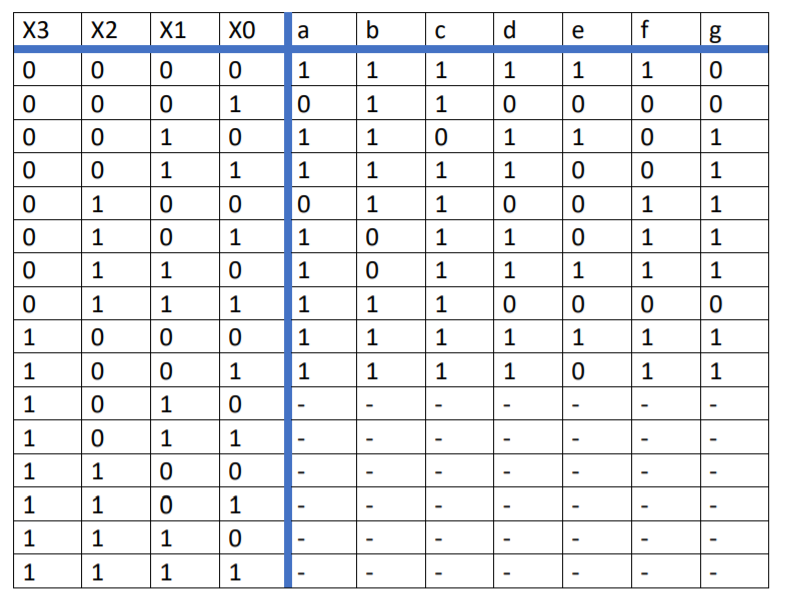
\includegraphics[width=1\textwidth]{TablicaFunkcji.png}
\end{figure}
\section{Metoda tablic Karnaugha dla 1}
\subsection{Dla diody b}
\begin{figure}[H]
	\centering
	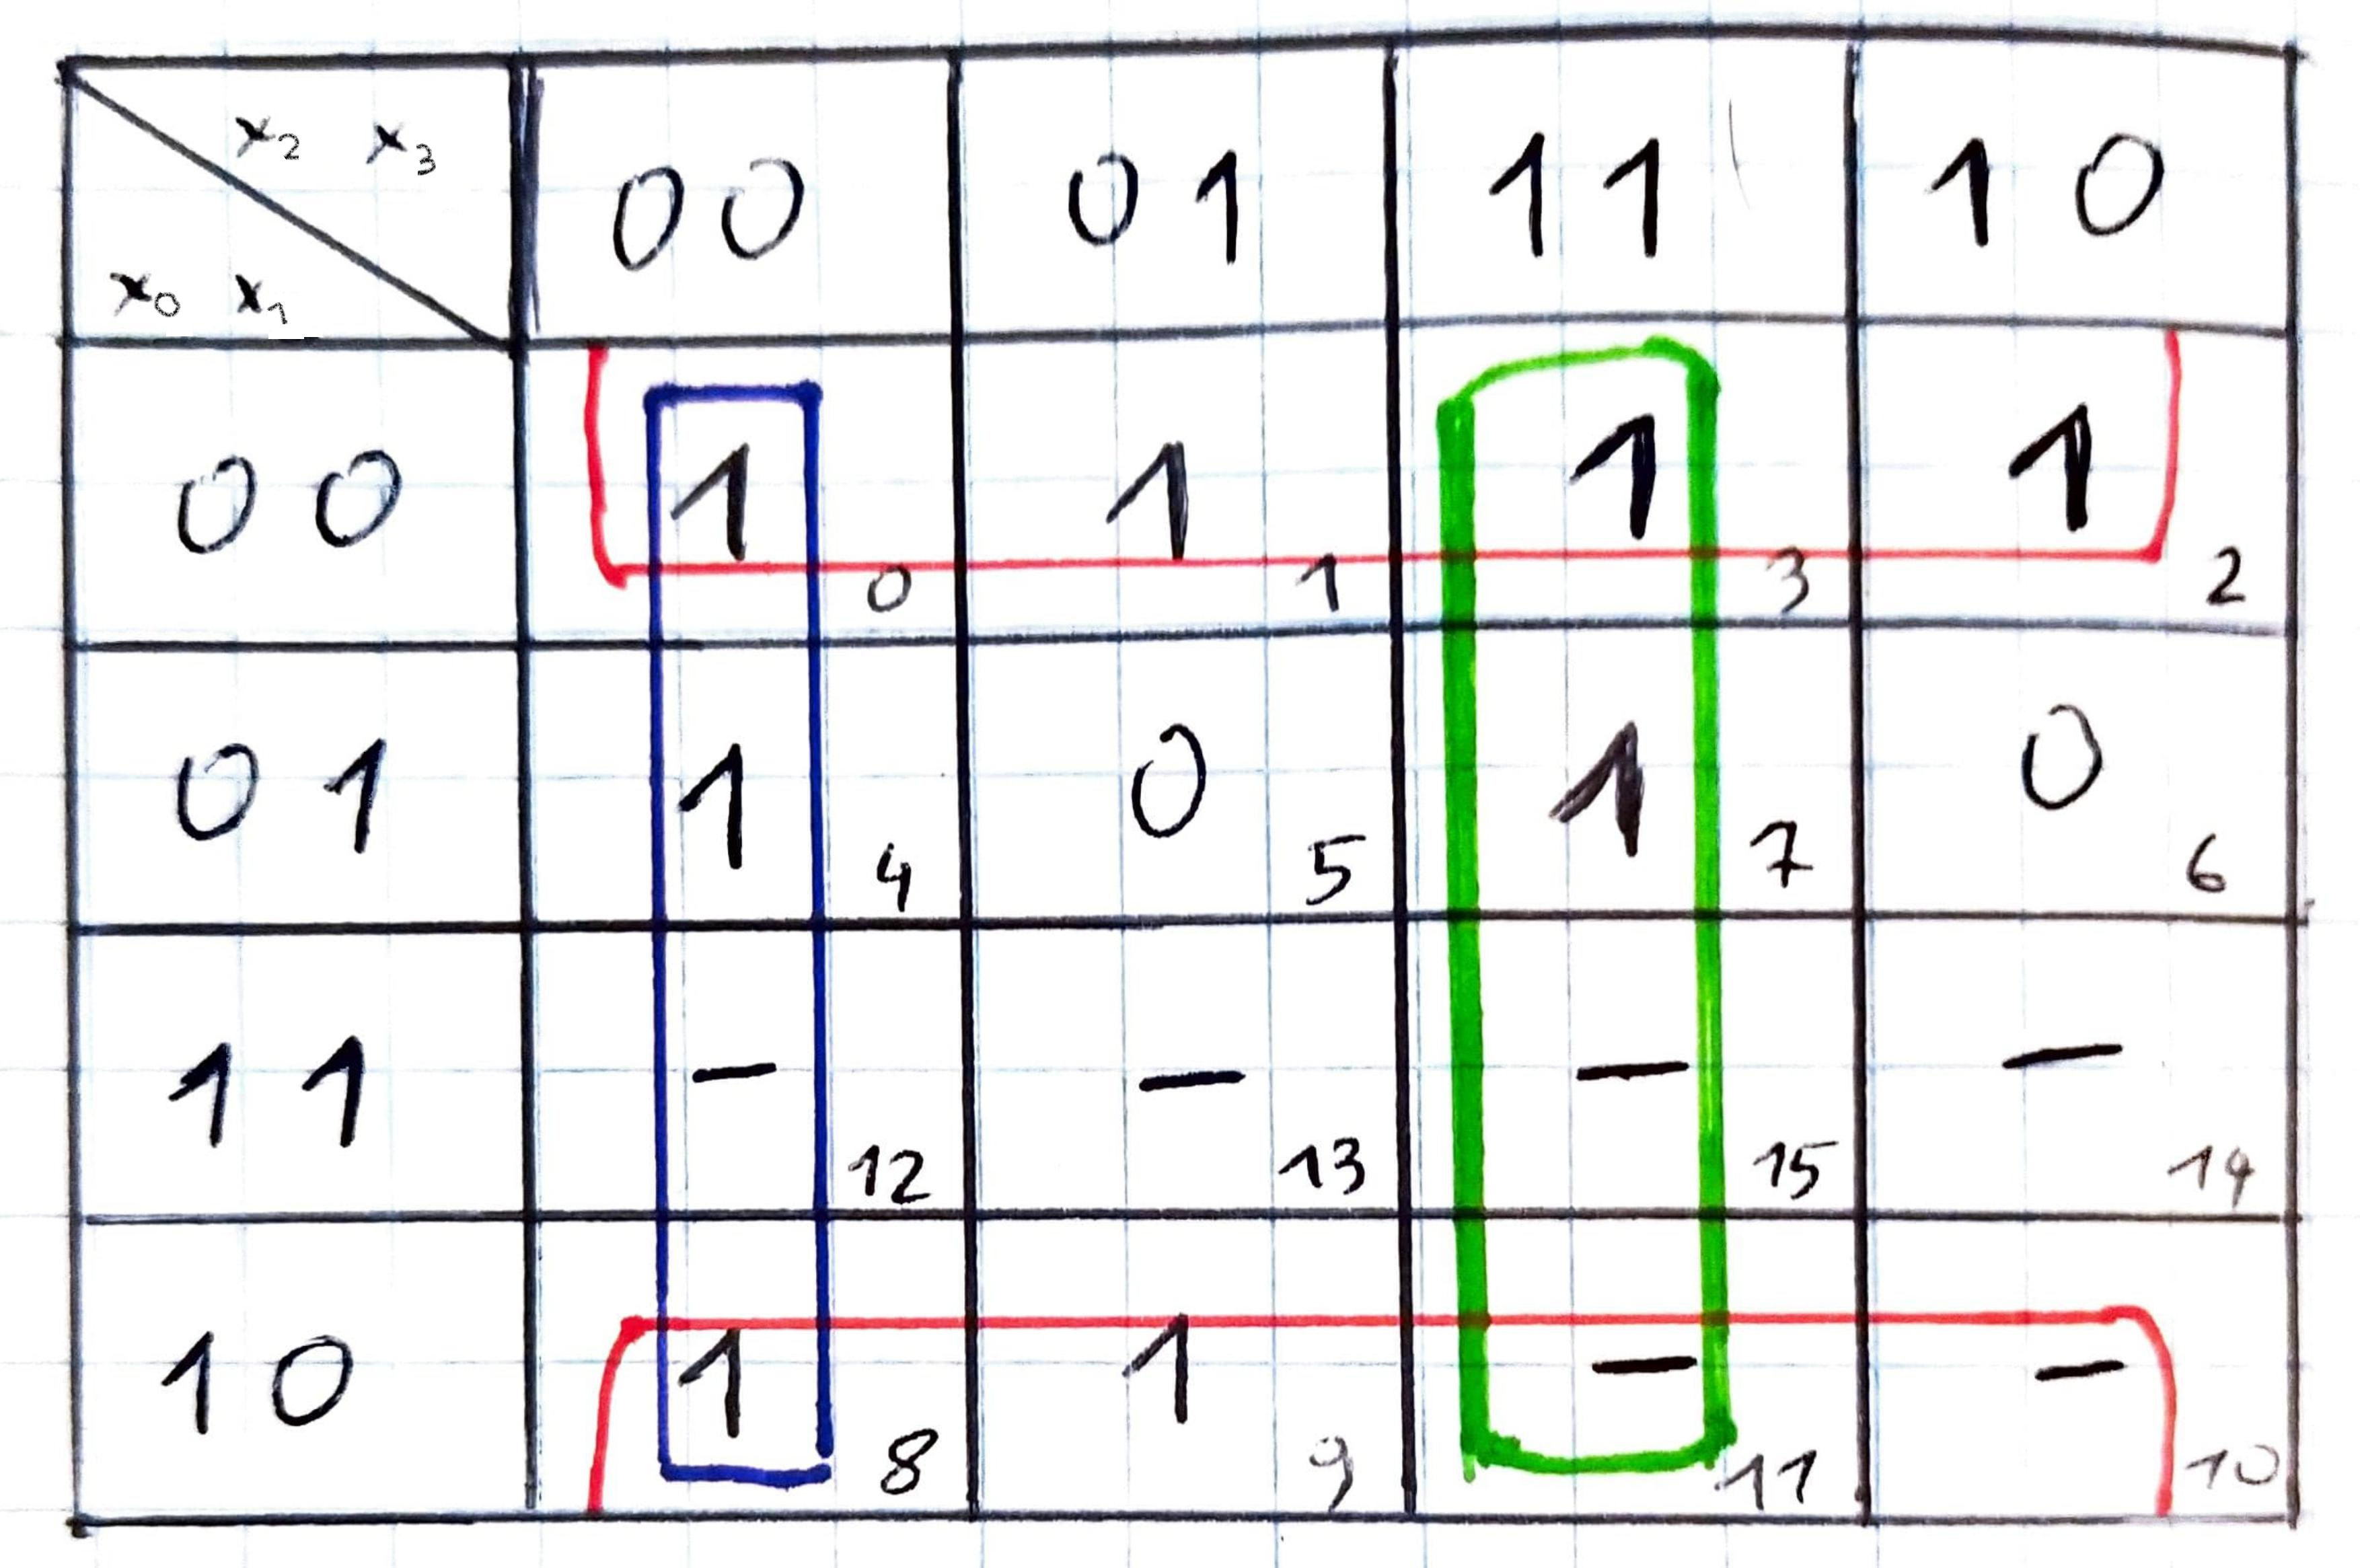
\includegraphics[width=1\textwidth]{minimalizacja_b.jpg}
\end{figure}
\textbf{SOP}: $b =\overline{x_{1}}+\overline{x_{2}}\overline{x_{3}}+x_{2}x_{3}$
\section{Metoda tablic Karnaugha dla 0}
\subsection{Dla diody c}
(Oznaczenia: $A=x_{3}, B=x_{2}, C=x_{1}, D=x_{0}$.)
\begin{figure}[H]
	\centering
	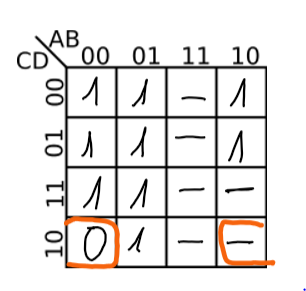
\includegraphics{c.png}
\end{figure}
\textbf{POS}: $c = (\overline{C}+B+D)=(x_{0}+\overline{x_{1}}+x_{2})$
\subsection{Dla diody d}
(Oznaczenia: $A=x_{3}, B=x_{2}, C=x_{1}, D=x_{0}$.)
\begin{figure}[H]
	\centering
	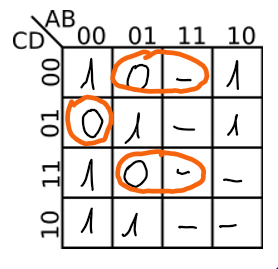
\includegraphics{d.png}
\end{figure}
\textbf{POS}: $d = (\overline{B}+C+D)(\overline{B}+\overline{C}+\overline{D})(A+B+C+\overline{D})=\\=(x_{0}+x_{1}+\overline{x_{2}})(\overline{x_{0}}+\overline{x_{1}}+\overline{x_{2}})
(\overline{x_{0}}+x_{1}+x_{2}+x_{3})$
\newpage
\section{Ekspansja systematyczna}
\subsection{Dla diody e}
F=\{0, 2, 6, 8\}(1)   R=\{1, 3, 4, 5, 7, 9\}(0)
\newline
\newline
\begin{minipage}{0.5\textwidth}
\centering
\begin{tabular}{|c|c|}
\hline
k\textsubscript{0} & 0000 \\
k\textsubscript{1} & 0010 \\
k\textsubscript{2} & 0110 \\
k\textsubscript{3} & 1000 \\
\hline
\end{tabular}
\end{minipage}
\hfill
\begin{minipage}{0.5\textwidth}
\centering
\begin{tabular}[r]{|c|c|}
\hline
    R & 0001 \\
      & 0011 \\
      & 0100 \\
      & 0101 \\
      & 0111 \\
      & 1001 \\
\hline 
\end{tabular}
\end{minipage}
\newline
\newline
\newline
k\textsubscript{0}=0000
\newline
Macierz blokująca
\newline
\begin{tabular}[r]{|c|c|}
\hline
    B\textsubscript{0} & 000\textcolor{red}{1} \\
      & \sout{0011} \\
      & \textcolor{red}{1}00 \\
      & \sout{0101} \\
      & \sout{0111} \\
      & \sout{1001} \\
 \hline 
\end{tabular}
\newline
\newline
\{L2,L0\}: I0 = (*0*0)
\newline
\newline
k\textsubscript{1}=0010
\newline
Macierz blokująca
\newline
\begin{tabular}[r]{|c|c|}
\hline
    B\textsubscript{1} & \sout{0011} \\
      & 000\textcolor{red}{1} \\
      & 0\textcolor{red}{1}\textcolor{red}{1}0 \\
      & \sout{0111} \\
      & \sout{0101} \\
      & \sout{1011} \\
 \hline 
\end{tabular}
\newline
\newline
\{L2,L0\} \{L1,L0\}: I1 = (*0*0), I2 = (**10)
\newline
\newline
k\textsubscript{2}=0110
\newline
Macierz blokująca
\newline
\begin{tabular}[r]{|c|c|}
\hline
    B\textsubscript{2} & \sout{0111} \\
      & \sout{0101} \\
      & 00\textcolor{red}{1}0 \\
      & \sout{0011} \\
      & 000\textcolor{red}{1} \\
      & \sout{1111} \\
\hline 
\end{tabular}
\newline
\newline
\{L4,L2\}: I3 = (**10)
\newpage
k\textsubscript{3}=1000
\newline
Macierz blokująca
\newline
\begin{tabular}[r]{|c|c|}
\hline
    B\textsubscript{3} & \sout{1001} \\
      & \sout{1011} \\
      & \textcolor{red}{1}\textcolor{red}{1}00 \\
      & \sout{1101} \\
      & \sout{1111} \\
      & 000\textcolor{red}{1} \\
 \hline 
\end{tabular}
\newline
\newline
\{L3,L0\} \{L2,L0\}: I4 = (1**0), I5 = (*0*0)
\newline
\newline
Wszystkie implikanty proste:
\newline
\newline
I0 = (*0*0), \sout{I1 = (*0*0)}, I2 = (**10), \sout{I3 = (**10)}, I4 = (1**0), \sout{I5 = (*0*0)}
\newline
\newline
\begin{tabular}[r]{|c|c|c|c|c|}
\hline
       &      & I0 = (*0*0) & I2 = (**10) & I4 = (1**0)\\
\hline
    k\textsubscript{0} & 0000 & \textcolor{red}{1} &   & \\
    k\textsubscript{1} & 0010 & \textcolor{red}{1} & \textcolor{red}{1} & \\
    k\textsubscript{2} & 0110 &   & \textcolor{red}{1} & \\
    k\textsubscript{3} & 1000 & \textcolor{red}{1} &   & 1 \\
 \hline 
\end{tabular}
\newline
\newline
$f(x\textsubscript{3},x\textsubscript{2},x\textsubscript{1},x\textsubscript{0}) = I0 + I2 = \overline{x_{2}}\overline{x_{0}} + x\textsubscript{1}\overline{x_{0}}$
\newpage
\subsection{Dla diody f}
F=\{0, 4, 5, 6, 8, 9\}(1)   R=\{1, 2, 3, 7\}(0)
\newline
\newline
\begin{minipage}{0.5\textwidth}
\centering
\begin{tabular}{|c|c|}
\hline
k0 & 0000 \\
k1 & 0100 \\
k2 & 0101 \\
k3 & 0110 \\
k4 & 1000 \\
k5 & 1001 \\
\hline
\end{tabular}
\end{minipage}
\hfill
\begin{minipage}{0.5\textwidth}
\centering
\begin{tabular}[r]{|c|c|}
\hline
    R & 0001 \\
      & 0010 \\
      & 0011 \\
      & 0111 \\
\hline 
\end{tabular}
\end{minipage}
\newline
\newline
\newline
k0=0000
\newline
Macierz blokująca
\newline
\begin{tabular}[r]{|c|c|}
\hline
    B0 & 000\textcolor{red}{1} \\
      & 00\textcolor{red}{1}0 \\
      & \sout{0011} \\
      & \sout{0111} \\
 \hline 
\end{tabular}
\newline
\newline
\{L1,L0\}: I0 = (**00)
\newline
\newline
k1=0100
\newline
Macierz blokująca
\newline
\begin{tabular}[r]{|c|c|}
\hline
    B1 & 0\textcolor{red}{1}0\textcolor{red}{1} \\
      & 0\textcolor{red}{1}\textcolor{red}{1}0 \\
      & \sout{0111} \\
      & 00\textcolor{red}{1}\textcolor{red}{1} \\
 \hline 
\end{tabular}
\newline
\newline
\{L2, L1\} \{L1, L0\}: I1 = (*10*), I2 = (**00)
\newline
\newline
k2=0101
\newline
Macierz blokująca
\newline
\begin{tabular}[r]{|c|c|}
\hline
    B2 & 0\textcolor{red}{1}00 \\
      & \sout{0111} \\
      & \sout{0110} \\
      & 00\textcolor{red}{1}0 \\
\hline 
\end{tabular}
\newline
\newline
\{L2,L1\}: I3 = (*10*)
\newpage
k3=0110
\newline
Macierz blokująca
\newline
\begin{tabular}[r]{|c|c|}
\hline
    B3 & \sout{0111} \\
      & 0\textcolor{red}{1}00 \\
      & \sout{0101} \\
      & 000\textcolor{red}{1} \\
 \hline 
\end{tabular}
\newline
\newline
\{L2,L0\}: I4 = (*1*0)
\newline
\newline
k4=1000
\newline
Macierz blokująca
\newline
\begin{tabular}[r]{|c|c|}
\hline
    B4 & \textcolor{red}{1}001 \\
      & \textcolor{red}{1}010 \\
      & \textcolor{red}{1}011 \\
      & \textcolor{red}{1}111 \\
\hline 
\end{tabular}
\newline
\newline
\{L3\}: I5 = (1***)
\newline
\newline
k5=1001
\newline
Macierz blokująca
\newline
\begin{tabular}[r]{|c|c|}
\hline
    B5 & \textcolor{red}{1}000 \\
      & \textcolor{red}{1}011 \\
      & \textcolor{red}{1}010 \\
      & \textcolor{red}{1}110 \\
\hline 
\end{tabular}
\newline
\newline
\{L3\}: I6 = (1***)
\newline
\newline
Wszystkie implikanty proste:
\newline
\newline
I0 = (**00), I1 = (*10*), \sout{I2 = (**00)}, \sout{I3 = (*10*)}, I4 = (*1*0), I5 = (1***), \sout{I6 = (1***)}
\newline
\newline
\begin{tabular}[r]{|c|c|c|c|c|c|}

\hline
       &      & I0 = (**00) & I1 = (*10*) & I4 = (*1*0) & I5 = (1***)\\
\hline
    k0 & 0000 & \textcolor{red}{1} &   &   &  \\
    k1 & 0100 & \textcolor{red}{1} & \textcolor{red}{1} & \textcolor{red}{1} &  \\
    k2 & 0101 &   & \textcolor{red}{1} &   &  \\
    k3 & 0110 &   &   & \textcolor{red}{1} &  \\
    k4 & 1000 & \textcolor{red}{1} &   &   & \textcolor{red}{1}\\
    k5 & 1001 &   &   &   & \textcolor{red}{1}\\
 \hline 
\end{tabular}
\newline
\newline
$f(x\textsubscript{3},x\textsubscript{2},x\textsubscript{1},x\textsubscript{0}) = I0 + I1 + I4 + I5 = \overline{x_{1}}\overline{x_{0}} + x\textsubscript{2}\overline{x_{1}} + x\textsubscript{2}\overline{x_{0}} + x\textsubscript{3}$
\newpage
\section{Ekspansja heurystyczna}
\subsection{Dla diody g}
F=\{2,3,4,5,6,8,9\}(1)   R=\{0,1,7\}(0)
\newline
\newline
\begin{minipage}{0.5\textwidth}
\centering
\begin{tabular}{|c|c|}
\hline
k0 & \fcolorbox{pink}{pink}{\sout{0010}} \\
k1 & \fcolorbox{pink}{pink}{\sout{0011}} \\
k2 & \fcolorbox{pink}{green}{\sout{0100}} \\
k3 & \fcolorbox{pink}{green}{\sout{0101}} \\
k4 & \fcolorbox{yellow}{yellow}{\sout{0110}} \\
k5 & \fcolorbox{yellow}{cyan}{\sout{1000}} \\
k6 & \fcolorbox{yellow}{cyan}{\sout{1001}} \\
\hline
\end{tabular}
\end{minipage}
\hfill
\begin{minipage}{0.5\textwidth}
\centering
\begin{tabular}[r]{|c|c|}
\hline
    R & 0000  \\
      & 0001 \\
      & 0111 \\
 \hline 
\end{tabular}
\end{minipage}
\newline
\newline
\newline
k0=0010
\newline
Macierz blokująca
\newline
\begin{tabular}[r]{|c|c|}
\hline
    B0 & 00\textcolor{red}{1}0  \\
      & \sout{0011} \\
      & 0\textcolor{red}{1}0\textcolor{red}{1} \\
 \hline 
\end{tabular}
\newline
\newline
\{L2,L1\} \{L1,L0\}: \fcolorbox{pink}{pink}{I0 = (*01*)},I1 = (**10)
\newline
\newline
k1=0011
\newline
Macierz blokująca
\newline
\begin{tabular}[r]{|c|c|}
\hline
    B1 & \sout{0011}  \\
      & 00\textcolor{red}{1}0 \\
      & 0\textcolor{red}{1}00 \\
 \hline 
\end{tabular}
\newline
\newline
\{L2,L1\}: I2 = (*01*)
\newline
\newline
k2=0100
\newline
Macierz blokująca
\newline
\begin{tabular}[r]{|c|c|}
\hline
    B2 & 0\textcolor{red}{1}00   \\
      & \sout{0101} \\
      & 00\textcolor{red}{1}\textcolor{red}{1} \\
 \hline 
\end{tabular}
\newline
\newline
\{L2,L1\},\{L2,L0\}: \fcolorbox{pink}{green}{I3 = (*10*)}, I4 = (*1*0)
\newline
\newline
k3=0101
\newline
Macierz blokująca
\newline
\begin{tabular}[r]{|c|c|}
\hline
    B3 & \sout{0101}  \\
      & 0\textcolor{red}{1}00 \\
      & 00\textcolor{red}{1}0 \\
 \hline 
\end{tabular}
\newline
\newline
\{L2,L1\}: I5 = (*10*)
\newline
\newline
k4=0110
\newline
Macierz blokująca
\newline
\begin{tabular}[r]{|c|c|}
\hline
    B4 & 0\textcolor{red}{1}\textcolor{red}{1}0  \\
      & \sout{0111} \\
      & 000\textcolor{red}{1} \\
 \hline 
\end{tabular}
\newline
\newline
\{L2,L0\},\{L1,L0\}: \fcolorbox{yellow}{yellow}{I6 = (*1*0)}, I7=(**10)
\newline
\newline
k5=1000
\newline
Macierz blokująca
\newline
\begin{tabular}[r]{|c|c|}
\hline
    B5 & \textcolor{red}{1}000  \\
      & \sout{1001} \\
      & \sout{1111} \\
 \hline 
\end{tabular}
\newline
\newline
\{L3\}: \fcolorbox{yellow}{cyan}{I8 = (1***)}
\newline
\newline
k6=1001
\newline
Macierz blokująca
\newline
\begin{tabular}[r]{|c|c|}
\hline
    B6 & \sout{1001}  \\
      & \textcolor{red}{1}000 \\
      & \sout{1110} \\
 \hline 
\end{tabular}
\newline
\newline
\{L3\}: I9 = (1***)
\newline
\newline
$f(x\textsubscript{3},x\textsubscript{2},x\textsubscript{1},x\textsubscript{0})= I0 + I3 + I6 + I8 = \overline{x_{2}}x\textsubscript{1} + x\textsubscript{2}\overline{x_{1}} +x\textsubscript{2}\overline{x_{0}} + x\textsubscript{3}$
\subsection{Dla diody a}
F=\{0,2,3,5,6,7,8,9\}(1)   R=\{1,4\}(0)
\newline
\newline
\begin{minipage}{0.5\textwidth}
\centering
\begin{tabular}[]{|c|c|}
\hline
    k0 & \fcolorbox{pink}{yellow}{\sout{0000}} \\
    k1 & \fcolorbox{pink}{yellow}{\sout{0010}} \\
    k2 & \fcolorbox{pink}{pink}{\sout{0011}} \\
    k3 & \fcolorbox{pink}{green}{\sout{0101}} \\
    k4 & \fcolorbox{yellow}{pink}{\sout{0110}} \\
    k5 & \fcolorbox{yellow}{pink}{\sout{0111}} \\
    k6 & \fcolorbox{yellow}{yellow}{\sout{1000}} \\
    k7 & \fcolorbox{yellow}{cyan}{\sout{1001}} \\
    \hline
\end{tabular}
\end{minipage}
\hfill
\begin{minipage}{0.5\textwidth}
\centering
\begin{tabular}[r]{|c|c|}
\hline
    R & 0001  \\
      & 0100 \\
 \hline 
\end{tabular}
\end{minipage}
\newline
\newline
\newline
k0=0000
\newline
Macierz blokująca
\newline
\begin{tabular}[r]{|c|c|}
\hline
    B0 & 000\textcolor{red}{1}  \\
      & 0\textcolor{red}{1}00 \\
 \hline 
\end{tabular}
\newline
\newline
\{L2,L0\}: \fcolorbox{pink}{yellow}{I0 = (*0*0)}
\newline
\newline
k1=0010
\newline
Macierz blokująca
\newline
\begin{tabular}[r]{|c|c|}
\hline
    B1 & 00\textcolor{red}{1}\textcolor{red}{1}  \\
      & 0\textcolor{red}{1}\textcolor{red}{1}0 \\
      
 \hline 
\end{tabular}
\newline
\newline
\{L2,L1,L0\}: I1 = (*010)
\newline
\newline
k2=0011
\newline
Macierz blokująca
\newline
\begin{tabular}[r]{|c|c|}
\hline
    B2 & 00\textcolor{red}{1}0   \\
      & \sout{0111} \\
 \hline 
\end{tabular}
\newline
\newline
\{L2\}: \fcolorbox{pink}{pink}{I2 = (**1*)}
\newline
\newline
k3=0101
\newline
Macierz blokująca
\newline
\begin{tabular}[r]{|c|c|}
\hline
    B3 &  0\textcolor{red}{1}00 \\
      & 000\textcolor{red}{1} \\
 \hline 
\end{tabular}
\newline
\newline
\{L2,L0\}: \fcolorbox{pink}{green}{I3 = (*1*1)}
\newline
\newline
k4=0110
\newline
Macierz blokująca
\newline
\begin{tabular}[r]{|c|c|}
\hline
    B4 & \sout{0111} \\
      & 00\textcolor{red}{1}0 \\
 \hline 
\end{tabular}
\newline
\newline
\{L1\}: I4 = (**10)
\newline
\newline
k5=0111
\newline
Macierz blokująca
\newline
\begin{tabular}[r]{|c|c|}
\hline
    B5 & 00\textcolor{red}{1}0  \\
      & \sout{0111} \\
 \hline 
\end{tabular}
\newline
\newline
\{L1\}:I5 = (**1*)
\newline
\newline
k6=1000
\newline
Macierz blokująca
\newline
\begin{tabular}[r]{|c|c|}
\hline
    B6 & \textcolor{red}{1}00\textcolor{red}{1} \\
       & \textcolor{red}{1}\textcolor{red}{1}00 \\
 \hline 
\end{tabular}
\newline
\newline
\{L3,L2,L0\}: I6 = (10*0))
\newline
\newline
k7=1001
\newline
Macierz blokująca
\newline
\begin{tabular}[r]{|c|c|}
\hline
    B7 & \textcolor{red}{1}000 \\
       & \sout{1101} \\
 \hline 
\end{tabular}
\newline
\newline
\{L3\}: \fcolorbox{pink}{cyan}{I7 = (1***)}
\newline
\newline
$f(x\textsubscript{3},x\textsubscript{2},x\textsubscript{1},x\textsubscript{0})= I0 + I2 + I3 + I7 = \overline{x_{2}}\overline{x_{0}} + x\textsubscript{1} + x\textsubscript{2}x\textsubscript{0} + x\textsubscript{3}$
\section{Logisim}
\subsection{Układ bramkowy}
\begin{figure}[H]
	\centering
	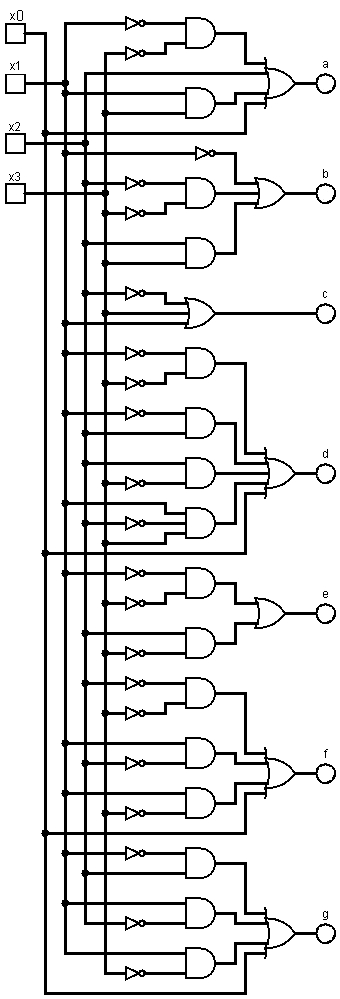
\includegraphics[width=0.5\textwidth]{uklad_bramkowy.png}
\end{figure}
\subsection{Testy}
Input:0000
\begin{figure}[H]
	\centering
	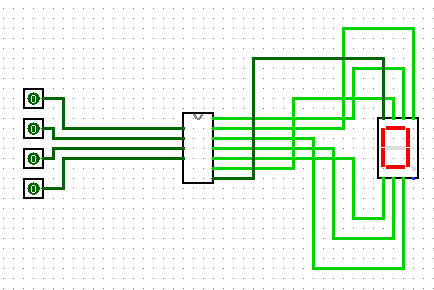
\includegraphics[width=0.65\textwidth]{0.png}
\end{figure}
Input:0001
\begin{figure}[H]
	\centering
	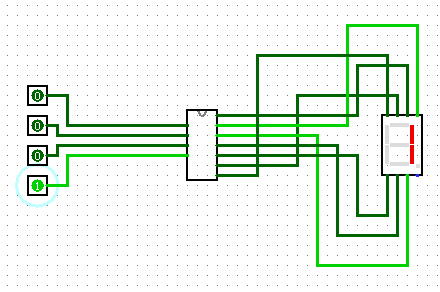
\includegraphics[width=0.65\textwidth]{1.png}
\end{figure}
Input:0010
\begin{figure}[H]
	\centering
	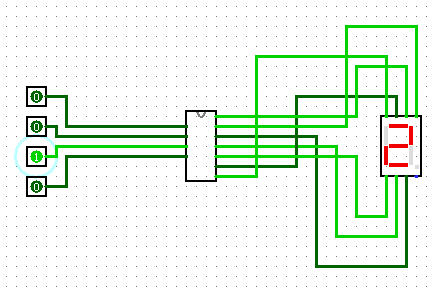
\includegraphics[width=0.65\textwidth]{2.png}
\end{figure}
Input:0011
\begin{figure}[H]
	\centering
	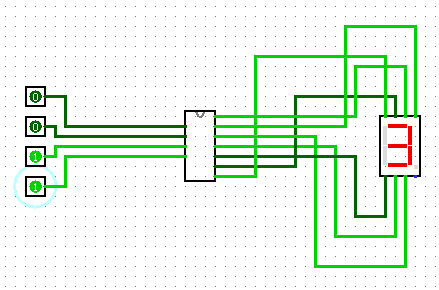
\includegraphics[width=0.65\textwidth]{3.png}
\end{figure}
Input:0100
\begin{figure}[H]
	\centering
	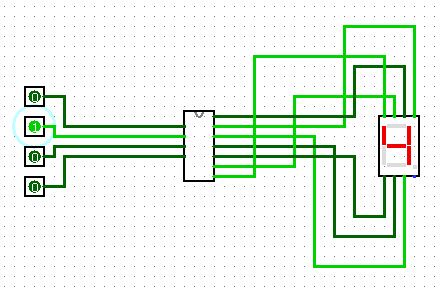
\includegraphics[width=0.65\textwidth]{4.png}
\end{figure}
Input:0101
\begin{figure}[H]
	\centering
	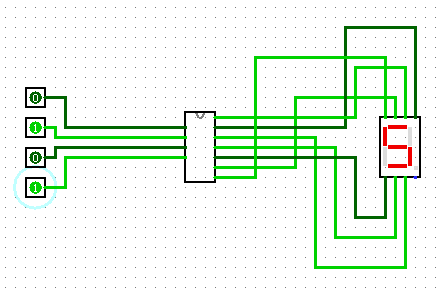
\includegraphics[width=0.65\textwidth]{5.png}
\end{figure}
Input:0110
\begin{figure}[H]
	\centering
	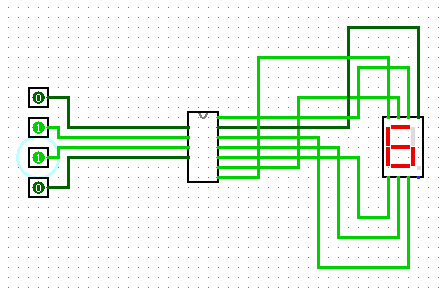
\includegraphics[width=0.65\textwidth]{6.png}
\end{figure}
Input:0111
\begin{figure}[H]
	\centering
	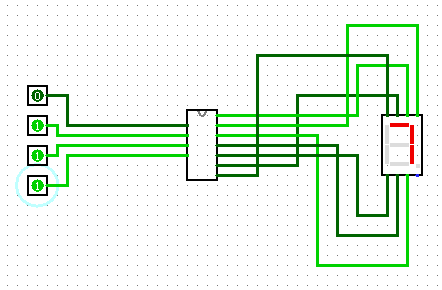
\includegraphics[width=0.65\textwidth]{7.png}
\end{figure}
Input:1000
\begin{figure}[H]
	\centering
	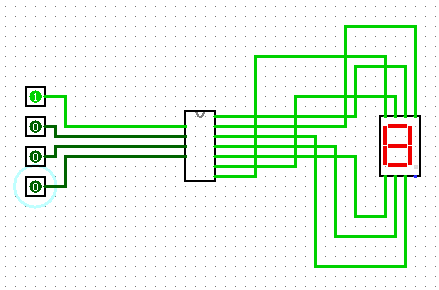
\includegraphics[width=0.65\textwidth]{8.png}
\end{figure}
Input:1001
\begin{figure}[H]
	\centering
	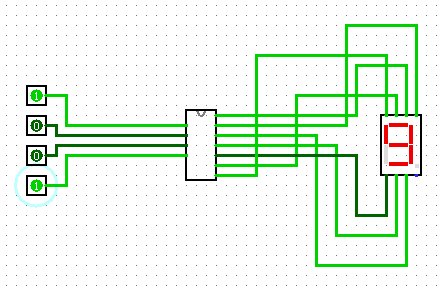
\includegraphics[width=0.65\textwidth]{9.png}
\end{figure}
\end{document}
